% ============================================================================
% CSCE 763: Digital Image Processing - Homework 2 Solutions
% ============================================================================

\documentclass[12pt]{article}

% ============================================================================
% PACKAGE IMPORTS
% ============================================================================
\usepackage{amsmath}
\usepackage{graphicx}
\usepackage{amssymb}
\usepackage{tikz}
\usepackage[margin=1in]{geometry}
\usepackage{setspace}
\usepackage{xcolor}
\usepackage{enumitem}
\usepackage{tcolorbox}
\usepackage{fancyhdr}
\usepackage{booktabs}
\usepackage{array}
\usepackage{colortbl}
\usepackage{float}

% ============================================================================
% HEADER AND FOOTER SETUP
% ============================================================================
\pagestyle{fancy}
\setlength{\headheight}{14.5pt}
\fancyhf{}

\fancyhead[L]{Page \thepage}
\fancyhead[C]{CSCE 763}
\fancyhead[R]{JC Vaught}

\renewcommand{\headrulewidth}{0pt}

% ============================================================================
% TIKZ LIBRARIES
% ============================================================================
\usetikzlibrary{shapes.geometric, arrows.meta, positioning, patterns, calc}

% --- USC Brand Colors ---
\definecolor{USC_Garnet}{HTML}{73000A}
\definecolor{USC_Sandstorm}{HTML}{FFF2E3}
\definecolor{USC_Black90}{HTML}{363636}
\definecolor{USC_Black70}{HTML}{5C5C5C}
\definecolor{USC_Black50}{HTML}{A2A2A2}
\definecolor{USC_Black10}{HTML}{ECECEC}
\definecolor{USC_Honeycomb}{HTML}{65780B}
\definecolor{USC_Atlantic}{HTML}{466A9F}
\definecolor{USC_Congaree}{HTML}{1F414D}
\definecolor{USC_Rose}{HTML}{CC2E40}
\definecolor{USC_Grass}{HTML}{CED318}
\definecolor{USC_Horseshoe}{HTML}{65780B}
\definecolor{outputbg}{RGB}{245,245,245}

% ============================================================================
% CUSTOM COLORED BOXES
% ============================================================================
\newtcolorbox{stepbox}[1][Step]{
  colback=white,
  colframe=USC_Garnet,
  fonttitle=\bfseries,
  title=#1,
  sharp corners,
  colbacktitle=USC_Garnet,
  coltitle=white,
}

\newtcolorbox{resultsbox}{
  colback=white,
  colframe=USC_Honeycomb,
  fonttitle=\bfseries,
  title=Results,
  sharp corners,
  colbacktitle=USC_Honeycomb,
  coltitle=white,
}

% ============================================================================
% CUSTOM QUESTION AND PART COMMANDS
% ============================================================================
\newcommand{\question}[1]{%
  \clearpage
  \vspace{0.5cm}
  {\noindent\normalsize \textbf{#1}}
  \vspace{0.2cm}
  \hrule
  \vspace{0.1cm}
  \hrule
  \vspace{0.3cm}
}

\newcommand{\questionpart}[1]{%
  \clearpage
  \vspace{0.5cm}
  {\noindent\normalsize \textbf{#1}}
  \vspace{0.2cm}
  \hrule
  \vspace{0.1cm}
  \hrule
  \vspace{0.3cm}
}

% Graphics path
\graphicspath{{figures/}}

% ============================================================================
% DOCUMENT INFORMATION
% ============================================================================

\title{CSCE 763: Digital Image Processing \\ Homework \#2}
\author{Instructor: Spring 2026 \\ University of South Carolina \\ \textit{Solutions by: JC Vaught}}
\date{Due: 1:15 pm EST, Tuesday, Feb 10}

% ============================================================================
% BEGIN DOCUMENT
% ============================================================================

\begin{document}

\maketitle
\setlength{\parindent}{0pt}

\setlist[enumerate,1]{label=\arabic*.}
\setlist[enumerate,2]{label=(\alph*)}

% ============================================================================
% TABLE OF CONTENTS
% ============================================================================

\begin{center}
\begin{tcolorbox}[colback=white, colframe=gray!50!black, colbacktitle=gray!20!white,
                  coltitle=black, sharp corners, boxrule=1pt,
                  title=\Large\bfseries Table of Contents]
\begin{tabular}{p{0.82\textwidth}r}
\textbf{Problem 1: Median Operator Nonlinearity (10 pts)} \dotfill & \textbf{\pageref{quest:1}} \\[0.3em]
\textbf{Problem 2: Image Subtraction for Defect Detection (20 pts)} \dotfill & \textbf{\pageref{quest:2}} \\[0.3em]
\textbf{Problem 3: Histogram Equalization Idempotency (20 pts)} \dotfill & \textbf{\pageref{quest:3}} \\[0.3em]
\textbf{Problem 4: Histogram Matching (30 pts)} \dotfill & \textbf{\pageref{quest:4}} \\[0.3em]
\textbf{Problem 5: Continuous Intensity Transformation (20 pts)} \dotfill & \textbf{\pageref{quest:5}} \\
\end{tabular}
\vspace{0.2cm}
\end{tcolorbox}
\end{center}

\vspace{0.5cm}

% ============================================================================
% PROBLEM 1: Median Operator Nonlinearity
% ============================================================================

\question{Problem 1: Median Operator Nonlinearity (10 pts)}\label{quest:1}

The median $\zeta$, of a set of numbers is such that half the values in the set are below $\zeta$, and the other half are above it. For example, the median of the set of values $\{12, 3, 8, 20, 21, 75, 31\}$ is 20. Show that an operator that computes the median of a subimage area, $S$, is nonlinear.

\textbf{Hints:} an operator $H$ is linear if
\[
H[a_1 f_1(x,y) + a_2 f_2(x,y)] = a_1 H[f_1(x,y)] + a_2 H[f_2(x,y)]
\]

\vspace{0.5cm}

\begin{stepbox}[Step 1: State the Linearity Condition]
An operator $H$ is linear if and only if the \textbf{superposition property} holds for all images $f_1, f_2$ and all scalars $a_1, a_2$:
\[
H[a_1 f_1 + a_2 f_2] = a_1 H[f_1] + a_2 H[f_2]
\]
To show $H$ is nonlinear, it suffices to find a single counterexample where this equality fails. We set $a_1 = a_2 = 1$ and test the additivity property over a $1 \times 3$ subimage region $S$.
\end{stepbox}

\begin{stepbox}[Step 2: Define the Counterexample]
Choose two images defined by their pixel values over $S$:
\[
f_1 = \{2,\; 3,\; 10\}, \qquad f_2 = \{10,\; 1,\; 2\}
\]
\end{stepbox}

\begin{stepbox}[Step 3: Compute the Right-Hand Side]
\[
H[f_1] + H[f_2] = \text{median}\{2,3,10\} + \text{median}\{10,1,2\} = 3 + 2 = 5
\]
\end{stepbox}

\begin{stepbox}[Step 4: Compute the Left-Hand Side]
\[
f_1 + f_2 = \{2+10,\; 3+1,\; 10+2\} = \{12,\; 4,\; 12\}
\]
\[
H[f_1 + f_2] = \text{median}\{12, 4, 12\} = 12
\]
\end{stepbox}

\begin{stepbox}[Step 5: Conclude]
Since
\[
H[f_1 + f_2] = 12 \neq 5 = H[f_1] + H[f_2]
\]
the superposition property is violated. Therefore, the median operator is \textbf{nonlinear}. $\blacksquare$
\end{stepbox}

\begin{stepbox}[Visualization: Counterexample Bar Chart]
\begin{center}
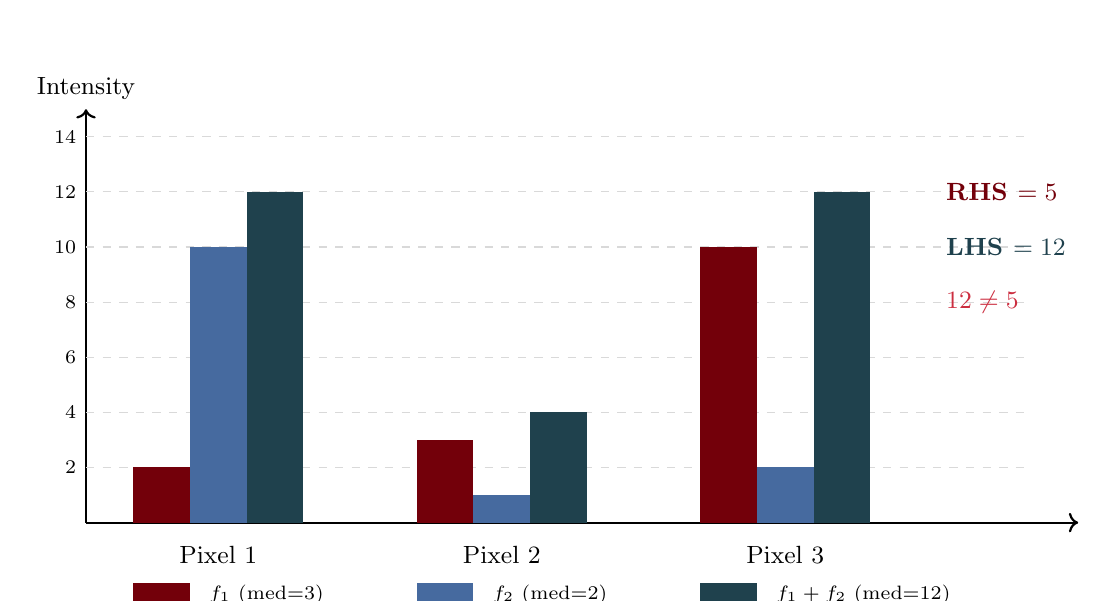
\begin{tikzpicture}[yscale=0.35, xscale=1.2]
% Axes
\draw[->, thick] (0,0) -- (10.5,0);
\draw[->, thick] (0,0) -- (0,15) node[above, font=\small] {Intensity};
% Y gridlines
\foreach \y in {2,4,6,8,10,12,14} {
  \draw[dashed, gray!30] (0,\y) -- (10,\y);
  \node[left, font=\scriptsize] at (0,\y) {\y};
}
% Bar groups: 3 pixels, 3 bars each
% Pixel 1
\fill[USC_Garnet] (0.5,0) rectangle (1.1,2);
\fill[USC_Atlantic] (1.1,0) rectangle (1.7,10);
\fill[USC_Congaree] (1.7,0) rectangle (2.3,12);
\node[below, font=\small] at (1.4,-0.5) {Pixel 1};
% Pixel 2
\fill[USC_Garnet] (3.5,0) rectangle (4.1,3);
\fill[USC_Atlantic] (4.1,0) rectangle (4.7,1);
\fill[USC_Congaree] (4.7,0) rectangle (5.3,4);
\node[below, font=\small] at (4.4,-0.5) {Pixel 2};
% Pixel 3
\fill[USC_Garnet] (6.5,0) rectangle (7.1,10);
\fill[USC_Atlantic] (7.1,0) rectangle (7.7,2);
\fill[USC_Congaree] (7.7,0) rectangle (8.3,12);
\node[below, font=\small] at (7.4,-0.5) {Pixel 3};
% Legend
\fill[USC_Garnet] (0.5,-3) rectangle (1.1,-2.2); \node[right, font=\scriptsize] at (1.2,-2.6) {$f_1$ (med$=$3)};
\fill[USC_Atlantic] (3.5,-3) rectangle (4.1,-2.2); \node[right, font=\scriptsize] at (4.2,-2.6) {$f_2$ (med$=$2)};
\fill[USC_Congaree] (6.5,-3) rectangle (7.1,-2.2); \node[right, font=\scriptsize] at (7.2,-2.6) {$f_1+f_2$ (med$=$12)};
% Annotations
\node[anchor=west, text=USC_Garnet, font=\small\bfseries] at (9,12) {RHS $= 5$};
\node[anchor=west, text=USC_Congaree, font=\small\bfseries] at (9,10) {LHS $= 12$};
\node[anchor=west, text=USC_Rose, font=\small\bfseries] at (9,8) {$12 \neq 5$};
\end{tikzpicture}
\end{center}
\end{stepbox}

\begin{resultsbox}
The median operator is \textbf{nonlinear}. The counterexample $f_1 = \{2, 3, 10\}$, $f_2 = \{10, 1, 2\}$ yields:
\[
H[f_1 + f_2] = 12 \neq 5 = H[f_1] + H[f_2] \qquad \blacksquare
\]
\end{resultsbox}


% ============================================================================
% PROBLEM 2: Image Subtraction
% ============================================================================

\question{Problem 2: Image Subtraction for Defect Detection (20 pts)}\label{quest:2}

Image subtraction is used often in industrial applications for detecting missing components in product assembly. The approach is to store a ``golden'' image that corresponds to a correct assembly; this image is then subtracted from incoming images of the same product. Ideally, the differences would be zero if the new products are assembled correctly. Difference images for products with missing components would be nonzero in the area where they differ from the golden image. What conditions do you think have to be met in practice for this method to work? You need to list at least two major factors that affect the detection performance.

\vspace{0.5cm}

To demonstrate these factors concretely, I applied various perturbations to a ``golden'' reference image of an industrial product (a pharmaceutical tablet) and computed the resulting difference images. Figure~\ref{fig:golden_image} shows the golden reference image used for this analysis.

\begin{figure}[H]
\centering
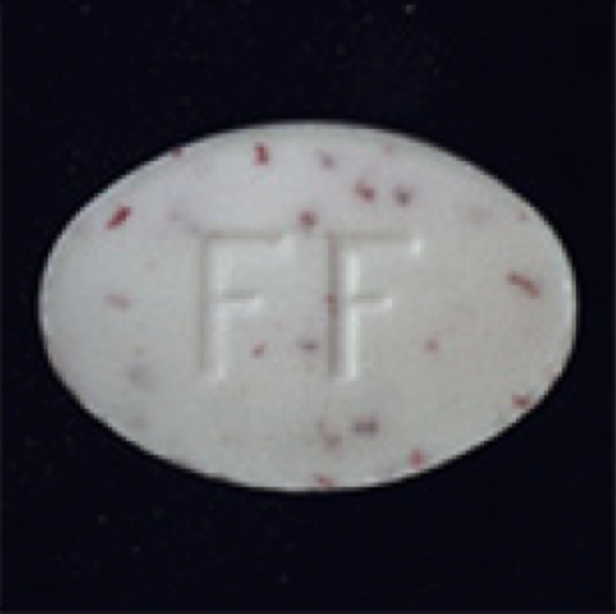
\includegraphics[width=0.35\textwidth]{example_golden.png}
\caption{Golden reference image of a pharmaceutical tablet with ``FF'' marking, used as the baseline for defect detection analysis.}
\label{fig:golden_image}
\end{figure}

\begin{stepbox}[Factor 1: Illumination Intensity]
Changes in overall lighting intensity cause uniform brightness shifts between images. Even small changes ($\pm 40$ intensity levels) produce significant difference signals across the entire image, creating false positives that completely mask actual defects.

\textbf{Practical requirement:} Fixed, calibrated light sources in enclosed inspection chambers.
\end{stepbox}

\begin{stepbox}[Factor 2: Spatial Translation]
If the product shifts position between captures---even by a few pixels---edges and high-contrast features produce large differences at boundaries. A 5-pixel shift creates false positives along all edges of the product.

\textbf{Practical requirement:} Mechanical fixtures, conveyor registration, or sub-pixel image alignment algorithms.
\end{stepbox}

\begin{stepbox}[Factor 3: Rotational Misalignment]
Angular misalignment (even 2°) causes the entire image to differ at every edge location. The difference pattern forms an arc around the object perimeter, which could easily be confused with circular defects.

\textbf{Practical requirement:} Rotational alignment fixtures or automated rotation correction.
\end{stepbox}

\begin{stepbox}[Factor 4: Scale/Zoom Variation]
Changes in camera-to-object distance or zoom settings alter the apparent size of the product. A 3\% scale change creates significant differences throughout the image, especially near edges.

\textbf{Practical requirement:} Fixed focal length, fixed working distance, or scale normalization preprocessing.
\end{stepbox}

\begin{stepbox}[Factor 5: Sensor Noise]
Random sensor noise ($\sigma = 20$ Gaussian) creates speckle-like differences uniformly distributed across the image. While individual noise pixels may be below threshold, accumulated noise raises the detection floor.

\textbf{Practical requirement:} Low-noise sensors, temporal averaging, or adaptive thresholding.
\end{stepbox}

\begin{stepbox}[Factor 6: Focus Blur]
If the test image is slightly out of focus compared to the golden image, edge sharpness differs. Blurring reduces edge contrast, creating differences where edges become softer.

\textbf{Practical requirement:} Auto-focus locks, fixed-focus telecentric lenses, or depth-of-field control.
\end{stepbox}

\begin{stepbox}[Factor 7: Non-uniform Illumination (Vignetting)]
Optical vignetting or uneven light distribution causes the image corners/edges to be darker than the center. This creates a characteristic radial difference pattern.

\textbf{Practical requirement:} Flat-field correction, uniform light sources, or calibrated vignetting correction.
\end{stepbox}

\begin{stepbox}[Factor 8: Contrast/Gain Variation]
Changes in camera gain or lighting contrast affect the dynamic range of the captured image. A 30\% contrast change produces differences proportional to local intensity.

\textbf{Practical requirement:} Fixed camera settings, calibrated exposure, auto-gain disabled.
\end{stepbox}

\begin{stepbox}[Factor 9: Color Temperature / White Balance]
Shifts in lighting color temperature (e.g., warm vs. cool) or white balance settings cause color channel differences. In grayscale conversion, this manifests as intensity shifts.

\textbf{Practical requirement:} Fixed white balance, controlled spectrum lighting (LED with fixed CCT).
\end{stepbox}

\begin{stepbox}[Factor 10: Perspective Distortion]
Changes in viewing angle create trapezoidal distortions. Even a 5\% perspective shift causes significant geometric differences, especially near image edges.

\textbf{Practical requirement:} Telecentric optics, fixed camera mount, perspective calibration.
\end{stepbox}

\begin{stepbox}[Factor 11: Exposure Variation]
Changes in exposure time (measured in EV stops) shift the overall image brightness non-linearly. Overexposure saturates bright regions while underexposure loses shadow detail.

\textbf{Practical requirement:} Fixed shutter speed, controlled ambient light, exposure calibration.
\end{stepbox}

\begin{stepbox}[Factor 12: Directional Shadows]
Shadows cast by external objects or non-uniform lighting create localized intensity variations. These appear as gradient differences across the image.

\textbf{Practical requirement:} Diffuse lighting, light tents, shadow-free illumination geometry.
\end{stepbox}

\vspace{0.5cm}

Figure~\ref{fig:failure_summary} shows a summary of six key failure modes applied to the golden image. Each column shows: (1) the perturbed test image, (2) the resulting difference image (brighter = larger difference), and (3) the false positives detected at a fixed threshold. Notice how environmental variations that leave the product physically unchanged still trigger significant detection artifacts.

\begin{figure}[H]
\centering

\includegraphics[width=\textwidth]{figures/failure_modes_summary.png}
\caption{Summary of failure modes in image subtraction detection. Row 1: Test images with various perturbations. Row 2: Difference images (hotter = larger difference). Row 3: Detected regions at threshold $T=30$. All perturbations produce false positives despite no actual defects.}
\label{fig:failure_summary}
\end{figure}

\vspace{0.5cm}

Figure~\ref{fig:failure_comparison} quantitatively compares all twelve failure modes by mean absolute difference. The key insight is that \textbf{illumination-related factors dominate}: brightness changes and exposure variations cause the largest false positive signals. Geometric factors (translation, rotation, scale) cause smaller mean differences but concentrate at edges where defects are often located. Critically, a true defect (missing component) has a relatively \textbf{small} mean difference because it affects only a localized region---demonstrating how failure modes can mask real defects.

\begin{figure}[H]
\centering
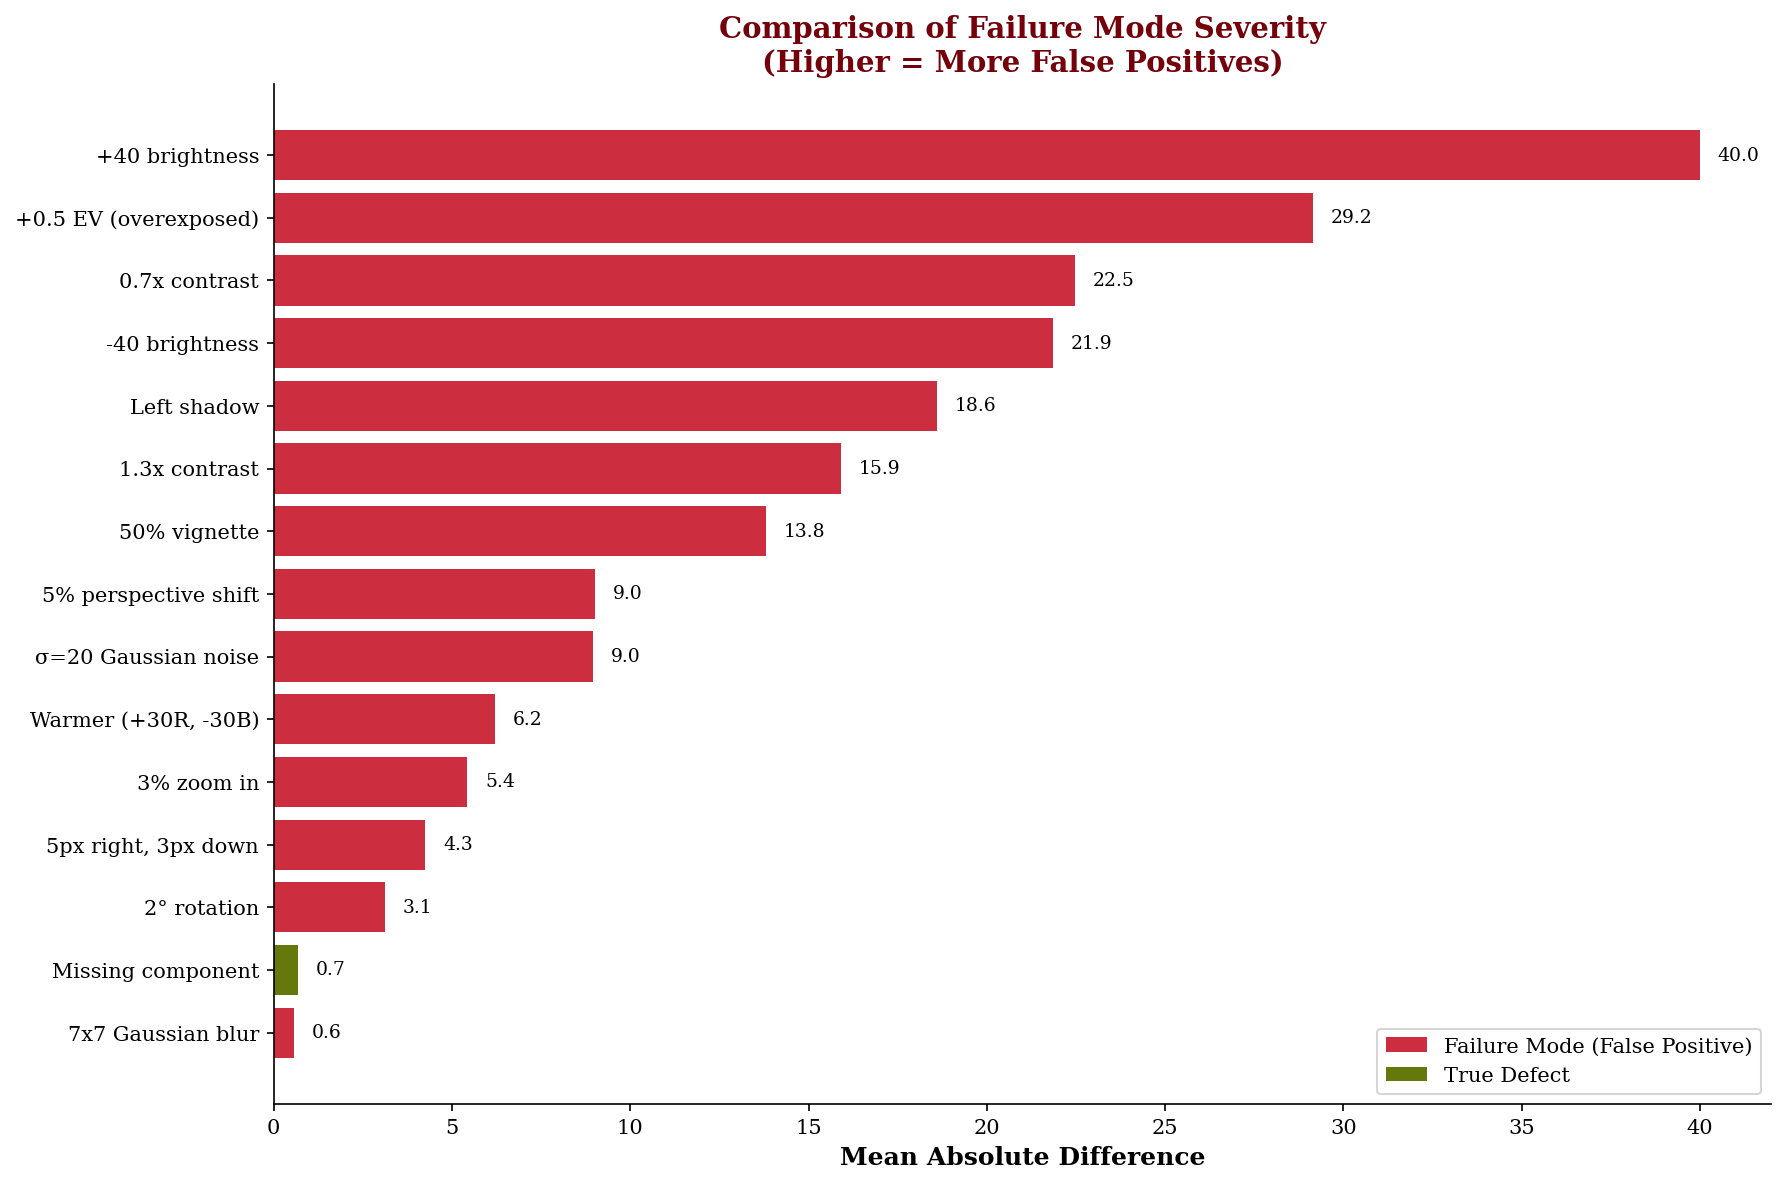
\includegraphics[width=0.9\textwidth]{figures/failure_modes_comparison.png}
\caption{Comparison of failure mode severity measured by mean absolute difference. Higher values indicate more false positives. Note that the true defect (missing component, green) has a \textit{lower} mean difference than most failure modes, illustrating how environmental variations can mask genuine defects.}
\label{fig:failure_comparison}
\end{figure}

\begin{resultsbox}
\textbf{Major factors affecting image subtraction defect detection:}

\vspace{0.2cm}
\textbf{Primary Factors (Must Control):}
\begin{enumerate}[leftmargin=*]
\item \textbf{Illumination consistency:} Intensity, direction, uniformity, and color temperature must be identical.
\item \textbf{Spatial registration:} Position, orientation, and scale must match exactly.
\end{enumerate}

\vspace{0.2cm}
\textbf{Secondary Factors (Should Control):}
\begin{enumerate}[leftmargin=*, start=3]
\item Sensor noise (requires thresholding)
\item Focus/sharpness consistency
\item Camera gain and exposure settings
\item White balance / color calibration
\item Perspective and optical distortion
\item Shadow elimination
\end{enumerate}

\vspace{0.2cm}
\textbf{Key insight:} Without controlling these factors, the mean difference from environmental variations can \textit{exceed} the difference caused by actual defects, making reliable detection impossible.
\end{resultsbox}


% ============================================================================
% PROBLEM 3: Histogram Equalization Idempotency
% ============================================================================

\question{Problem 3: Histogram Equalization Idempotency (20 pts)}\label{quest:3}

Suppose that a digital image is subjected to histogram equalization. Show that a second pass of histogram equalization (on the histogram-equalized image) will produce exactly the same result as the first pass.

\vspace{0.5cm}

\begin{stepbox}[Step 1: Define the Equalization Transform]
Let the original image have intensity levels $r \in [0, L-1]$ with PDF $p_r(r)$ and CDF $P_r(r)$. The histogram equalization transformation is:
\[
s = T(r) = (L-1)\, P_r(r) = (L-1) \int_0^r p_r(w)\, dw
\]
\end{stepbox}

\begin{stepbox}[Step 2: Show the Equalized Image Is Uniform]
A fundamental result from probability theory: if $s = T(r) = (L-1)\,P_r(r)$, then $s$ is \textbf{uniformly distributed} on $[0, L-1]$:
\[
p_s(s) = \frac{1}{L-1}, \qquad 0 \leq s \leq L-1
\]
\end{stepbox}

\begin{stepbox}[Step 3: Apply Equalization Again]
Apply histogram equalization a second time to the equalized image:
\[
v = T_2(s) = (L-1)\, P_s(s) = (L-1) \int_0^s p_s(w)\, dw
\]
Since $p_s(s) = \dfrac{1}{L-1}$, the CDF is:
\[
P_s(s) = \int_0^s \frac{1}{L-1}\, dw = \frac{s}{L-1}
\]
\end{stepbox}

\begin{stepbox}[Step 4: Simplify to Identity]
Substituting:
\[
v = T_2(s) = (L-1) \cdot \frac{s}{L-1} = s
\]
The second equalization is the \textbf{identity transformation}: $v = s$. The output is unchanged. $\blacksquare$
\end{stepbox}

\begin{stepbox}[Visualization: Histogram Through Two Equalization Passes]
\begin{center}
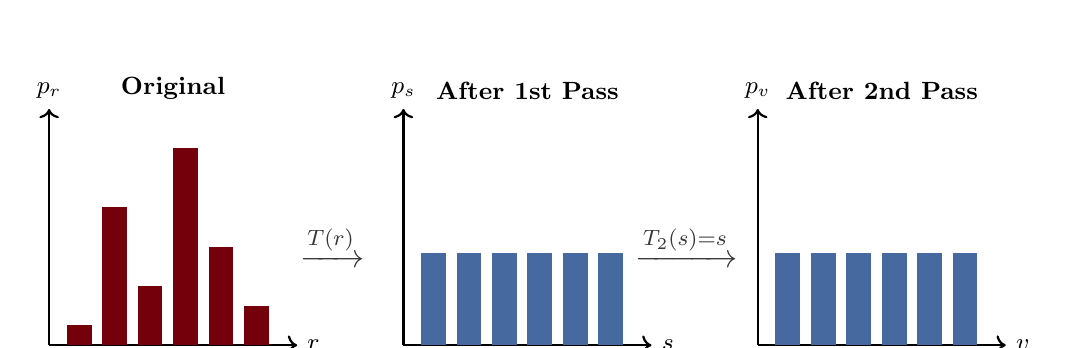
\begin{tikzpicture}[xscale=0.45, yscale=2.5]
% --- Panel 1: Original (arbitrary) ---
\begin{scope}[shift={(0,0)}]
\draw[->, thick] (0,0) -- (7,0) node[right, font=\small] {$r$};
\draw[->, thick] (0,0) -- (0,1.2) node[above, font=\small] {$p_r$};
\node[above, font=\small\bfseries] at (3.5,1.2) {Original};
\fill[USC_Garnet] (0.5,0) rectangle (1.2,0.1);
\fill[USC_Garnet] (1.5,0) rectangle (2.2,0.7);
\fill[USC_Garnet] (2.5,0) rectangle (3.2,0.3);
\fill[USC_Garnet] (3.5,0) rectangle (4.2,1.0);
\fill[USC_Garnet] (4.5,0) rectangle (5.2,0.5);
\fill[USC_Garnet] (5.5,0) rectangle (6.2,0.2);
\end{scope}
% Arrow 1
\node[font=\large, USC_Black90] at (8,0.5) {$\xrightarrow{T(r)}$};
% --- Panel 2: After 1st pass (uniform) ---
\begin{scope}[shift={(10,0)}]
\draw[->, thick] (0,0) -- (7,0) node[right, font=\small] {$s$};
\draw[->, thick] (0,0) -- (0,1.2) node[above, font=\small] {$p_s$};
\node[above, font=\small\bfseries] at (3.5,1.2) {After 1st Pass};
\foreach \x in {0.5,1.5,2.5,3.5,4.5,5.5} {
  \fill[USC_Atlantic] (\x,0) rectangle (\x+0.7,0.47);
}
\end{scope}
% Arrow 2
\node[font=\large, USC_Black90] at (18,0.5) {$\xrightarrow{T_2(s)=s}$};
% --- Panel 3: After 2nd pass (still uniform) ---
\begin{scope}[shift={(20,0)}]
\draw[->, thick] (0,0) -- (7,0) node[right, font=\small] {$v$};
\draw[->, thick] (0,0) -- (0,1.2) node[above, font=\small] {$p_v$};
\node[above, font=\small\bfseries] at (3.5,1.2) {After 2nd Pass};
\foreach \x in {0.5,1.5,2.5,3.5,4.5,5.5} {
  \fill[USC_Atlantic] (\x,0) rectangle (\x+0.7,0.47);
}
\end{scope}
\end{tikzpicture}
\end{center}
\end{stepbox}

\begin{resultsbox}
After the first histogram equalization, the output has a uniform distribution. Applying histogram equalization to a uniformly distributed image yields the identity mapping $v = s$. Therefore, the second pass produces exactly the same result as the first. $\blacksquare$
\end{resultsbox}


% ============================================================================
% PROBLEM 4: Histogram Matching
% ============================================================================

\question{Problem 4: Histogram Matching (30 pts)}\label{quest:4}

Suppose that a 4-bit image ($L=16$) of size $64 \times 64$ has the intensity distribution as Table~A. It is desired to transform the original histogram to a specified histogram as shown in Table~B. What will be the actual histogram after the histogram matching operation?

\vspace{0.5cm}

\begin{center}
\begin{minipage}{0.35\textwidth}
\centering
\rowcolors{2}{USC_Garnet!10}{white}
\begin{tabular}{>{\centering\arraybackslash}p{1.2cm} >{\centering\arraybackslash}p{1.2cm}}
\rowcolor{USC_Garnet!80}
\textcolor{white}{$r_k$} & \textcolor{white}{$n_k$} \\
\hline
0 & 16 \\
1 & 0 \\
2 & 512 \\
3 & 32 \\
4 & 64 \\
5 & 128 \\
6 & 64 \\
7 & 1024 \\
8 & 512 \\
9 & 512 \\
10 & 16 \\
11 & 1024 \\
12 & 0 \\
13 & 128 \\
14 & 0 \\
15 & 64 \\
\hline
\end{tabular}

\vspace{0.3cm}
\textbf{Table A}
\end{minipage}
\hspace{1cm}
\begin{minipage}{0.35\textwidth}
\centering
\rowcolors{2}{USC_Garnet!10}{white}
\begin{tabular}{>{\centering\arraybackslash}p{1.2cm} >{\centering\arraybackslash}p{1.2cm}}
\rowcolor{USC_Garnet!80}
\textcolor{white}{$z_q$} & \textcolor{white}{$n_q$} \\
\hline
0 & 64 \\
1 & 128 \\
2 & 512 \\
3 & 512 \\
4 & 1024 \\
5 & 1024 \\
6 & 512 \\
7 & 128 \\
8 & 128 \\
9 & 64 \\
10 & 0 \\
11 & 0 \\
12 & 0 \\
13 & 0 \\
14 & 0 \\
15 & 0 \\
\hline
\end{tabular}

\vspace{0.3cm}
\textbf{Table B}
\end{minipage}
\end{center}

\vspace{0.5cm}

\begin{stepbox}[Step 1: Setup]
Total pixels: $N = 64 \times 64 = 4096$, intensity levels: $L = 16$, so $L - 1 = 15$.

The equalization transform is:
\[
s_k = \text{round}\!\left(15 \cdot \sum_{j=0}^{k} \frac{n_j}{4096}\right)
\]
\end{stepbox}

\begin{stepbox}[Step 2: Cumulative Histogram and $s_k$ Values from Table A]
\begin{center}
\rowcolors{2}{USC_Garnet!10}{white}
\begin{tabular}{c c c c}
\rowcolor{USC_Garnet!80}
\textcolor{white}{$r_k$} & \textcolor{white}{$n_k$} & \textcolor{white}{$\displaystyle\sum_{j=0}^{k} n_j$} & \textcolor{white}{$s_k = \text{round}\!\left(\frac{15 \cdot \sum n_j}{4096}\right)$} \\
\hline
0  & 16   & 16   & $\text{round}(0.059) = 0$  \\
1  & 0    & 16   & $\text{round}(0.059) = 0$  \\
2  & 512  & 528  & $\text{round}(1.934) = 2$  \\
3  & 32   & 560  & $\text{round}(2.051) = 2$  \\
4  & 64   & 624  & $\text{round}(2.285) = 2$  \\
5  & 128  & 752  & $\text{round}(2.754) = 3$  \\
6  & 64   & 816  & $\text{round}(2.988) = 3$  \\
7  & 1024 & 1840 & $\text{round}(6.738) = 7$  \\
8  & 512  & 2352 & $\text{round}(8.613) = 9$  \\
9  & 512  & 2864 & $\text{round}(10.488) = 10$ \\
10 & 16   & 2880 & $\text{round}(10.547) = 11$ \\
11 & 1024 & 3904 & $\text{round}(14.297) = 14$ \\
12 & 0    & 3904 & $\text{round}(14.297) = 14$ \\
13 & 128  & 4032 & $\text{round}(14.766) = 15$ \\
14 & 0    & 4032 & $\text{round}(14.766) = 15$ \\
15 & 64   & 4096 & $\text{round}(15.000) = 15$ \\
\hline
\end{tabular}
\end{center}
\end{stepbox}

\begin{stepbox}[Step 3: Cumulative Histogram and $G(z_q)$ Values from Table B]
\begin{center}
\rowcolors{2}{USC_Garnet!10}{white}
\begin{tabular}{c c c c}
\rowcolor{USC_Garnet!80}
\textcolor{white}{$z_q$} & \textcolor{white}{$n_q$} & \textcolor{white}{$\displaystyle\sum_{j=0}^{q} n_j$} & \textcolor{white}{$G(z_q) = \text{round}\!\left(\frac{15 \cdot \sum n_j}{4096}\right)$} \\
\hline
0  & 64   & 64   & $\text{round}(0.234) = 0$  \\
1  & 128  & 192  & $\text{round}(0.703) = 1$  \\
2  & 512  & 704  & $\text{round}(2.578) = 3$  \\
3  & 512  & 1216 & $\text{round}(4.453) = 4$  \\
4  & 1024 & 2240 & $\text{round}(8.203) = 8$  \\
5  & 1024 & 3264 & $\text{round}(11.953) = 12$ \\
6  & 512  & 3776 & $\text{round}(13.828) = 14$ \\
7  & 128  & 3904 & $\text{round}(14.297) = 14$ \\
8  & 128  & 4032 & $\text{round}(14.766) = 15$ \\
9  & 64   & 4096 & $\text{round}(15.000) = 15$ \\
10 & 0    & 4096 & 15 \\
11 & 0    & 4096 & 15 \\
12 & 0    & 4096 & 15 \\
13 & 0    & 4096 & 15 \\
14 & 0    & 4096 & 15 \\
15 & 0    & 4096 & 15 \\
\hline
\end{tabular}
\end{center}
\end{stepbox}

\begin{stepbox}[Step 4: Inverse Mapping $s_k \to z_q$]
For each value of $s_k$, find the smallest $z_q$ such that $G(z_q) \geq s_k$:

\begin{center}
\rowcolors{2}{USC_Garnet!10}{white}
\begin{tabular}{c c c c}
\rowcolor{USC_Garnet!80}
\textcolor{white}{$r_k$} & \textcolor{white}{$s_k$} & \textcolor{white}{Smallest $z_q$ with $G(z_q) \geq s_k$} & \textcolor{white}{$z_q$} \\
\hline
0  & 0  & $G(0) = 0 \geq 0$   & 0 \\
1  & 0  & $G(0) = 0 \geq 0$   & 0 \\
2  & 2  & $G(2) = 3 \geq 2$   & 2 \\
3  & 2  & $G(2) = 3 \geq 2$   & 2 \\
4  & 2  & $G(2) = 3 \geq 2$   & 2 \\
5  & 3  & $G(2) = 3 \geq 3$   & 2 \\
6  & 3  & $G(2) = 3 \geq 3$   & 2 \\
7  & 7  & $G(4) = 8 \geq 7$   & 4 \\
8  & 9  & $G(5) = 12 \geq 9$  & 5 \\
9  & 10 & $G(5) = 12 \geq 10$ & 5 \\
10 & 11 & $G(5) = 12 \geq 11$ & 5 \\
11 & 14 & $G(6) = 14 \geq 14$ & 6 \\
12 & 14 & $G(6) = 14 \geq 14$ & 6 \\
13 & 15 & $G(8) = 15 \geq 15$ & 8 \\
14 & 15 & $G(8) = 15 \geq 15$ & 8 \\
15 & 15 & $G(8) = 15 \geq 15$ & 8 \\
\hline
\end{tabular}
\end{center}
\end{stepbox}

\begin{stepbox}[Step 5: Build the Output Histogram]
Using the mapping $r_k \to z_q$ and the pixel counts $n_k$ from Table A:

\begin{center}
\rowcolors{2}{USC_Garnet!10}{white}
\begin{tabular}{c c l}
\rowcolor{USC_Garnet!80}
\textcolor{white}{Output $z_q$} & \textcolor{white}{Mapped from $r_k$} & \textcolor{white}{Pixel count} \\
\hline
0 & $r_0, r_1$              & $16 + 0 = 16$ \\
1 & ---                      & 0 \\
2 & $r_2, r_3, r_4, r_5, r_6$ & $512 + 32 + 64 + 128 + 64 = 800$ \\
3 & ---                      & 0 \\
4 & $r_7$                    & 1024 \\
5 & $r_8, r_9, r_{10}$      & $512 + 512 + 16 = 1040$ \\
6 & $r_{11}, r_{12}$         & $1024 + 0 = 1024$ \\
7 & ---                      & 0 \\
8 & $r_{13}, r_{14}, r_{15}$ & $128 + 0 + 64 = 192$ \\
9--15 & ---                  & 0 each \\
\hline
\multicolumn{2}{r}{\textbf{Total:}} & $16+800+1024+1040+1024+192 = 4096$ \checkmark \\
\end{tabular}
\end{center}
\end{stepbox}

\begin{stepbox}[Visualization: Input, Desired, and Actual Output Histograms]
\begin{center}
\begin{tikzpicture}[xscale=0.28, yscale=0.0038]
% Helper: draw a single histogram panel
% --- Panel 1: Input (Table A) ---
\begin{scope}[shift={(0,0)}]
\draw[->, thick] (-0.5,0) -- (16.5,0) node[right, font=\small] {$r_k$};
\draw[->, thick] (-0.5,0) -- (-0.5,1150);
\node[above, font=\small\bfseries] at (8,1150) {Input (Table A)};
\foreach \y in {256,512,768,1024} {
  \draw[dashed, gray!30] (0,\y) -- (16,\y);
  \node[left, font=\tiny] at (-0.5,\y) {\y};
}
% Bars: r_k -> n_k
\fill[USC_Garnet] (0,0) rectangle (0.7,16);
% r1=0 skip
\fill[USC_Garnet] (2,0) rectangle (2.7,512);
\fill[USC_Garnet] (3,0) rectangle (3.7,32);
\fill[USC_Garnet] (4,0) rectangle (4.7,64);
\fill[USC_Garnet] (5,0) rectangle (5.7,128);
\fill[USC_Garnet] (6,0) rectangle (6.7,64);
\fill[USC_Garnet] (7,0) rectangle (7.7,1024);
\fill[USC_Garnet] (8,0) rectangle (8.7,512);
\fill[USC_Garnet] (9,0) rectangle (9.7,512);
\fill[USC_Garnet] (10,0) rectangle (10.7,16);
\fill[USC_Garnet] (11,0) rectangle (11.7,1024);
% r12=0 skip
\fill[USC_Garnet] (13,0) rectangle (13.7,128);
% r14=0 skip
\fill[USC_Garnet] (15,0) rectangle (15.7,64);
\end{scope}
% --- Panel 2: Desired (Table B) ---
\begin{scope}[shift={(20,0)}]
\draw[->, thick] (-0.5,0) -- (16.5,0) node[right, font=\small] {$z_q$};
\draw[->, thick] (-0.5,0) -- (-0.5,1150);
\node[above, font=\small\bfseries] at (8,1150) {Desired (Table B)};
\foreach \y in {256,512,768,1024} {
  \draw[dashed, gray!30] (0,\y) -- (16,\y);
  \node[left, font=\tiny] at (-0.5,\y) {\y};
}
\fill[USC_Atlantic] (0,0) rectangle (0.7,64);
\fill[USC_Atlantic] (1,0) rectangle (1.7,128);
\fill[USC_Atlantic] (2,0) rectangle (2.7,512);
\fill[USC_Atlantic] (3,0) rectangle (3.7,512);
\fill[USC_Atlantic] (4,0) rectangle (4.7,1024);
\fill[USC_Atlantic] (5,0) rectangle (5.7,1024);
\fill[USC_Atlantic] (6,0) rectangle (6.7,512);
\fill[USC_Atlantic] (7,0) rectangle (7.7,128);
\fill[USC_Atlantic] (8,0) rectangle (8.7,128);
\fill[USC_Atlantic] (9,0) rectangle (9.7,64);
\end{scope}
% --- Panel 3: Actual Output ---
\begin{scope}[shift={(40,0)}]
\draw[->, thick] (-0.5,0) -- (16.5,0) node[right, font=\small] {$z_q$};
\draw[->, thick] (-0.5,0) -- (-0.5,1150);
\node[above, font=\small\bfseries] at (8,1150) {Actual Output};
\foreach \y in {256,512,768,1024} {
  \draw[dashed, gray!30] (0,\y) -- (16,\y);
  \node[left, font=\tiny] at (-0.5,\y) {\y};
}
\fill[USC_Congaree] (0,0) rectangle (0.7,16);
% z1=0
\fill[USC_Congaree] (2,0) rectangle (2.7,800);
% z3=0
\fill[USC_Congaree] (4,0) rectangle (4.7,1024);
\fill[USC_Congaree] (5,0) rectangle (5.7,1040);
\fill[USC_Congaree] (6,0) rectangle (6.7,1024);
% z7=0
\fill[USC_Congaree] (8,0) rectangle (8.7,192);
\end{scope}
\end{tikzpicture}
\end{center}
\end{stepbox}

\begin{resultsbox}
The actual output histogram after histogram matching is:

\begin{center}
\rowcolors{2}{USC_Garnet!10}{white}
\begin{tabular}{>{\centering\arraybackslash}p{1.2cm} >{\centering\arraybackslash}p{1.5cm}}
\rowcolor{USC_Garnet!80}
\textcolor{white}{$z_q$} & \textcolor{white}{$n_q^{\text{out}}$} \\
\hline
0  & 16 \\
1  & 0 \\
2  & 800 \\
3  & 0 \\
4  & 1024 \\
5  & 1040 \\
6  & 1024 \\
7  & 0 \\
8  & 192 \\
9  & 0 \\
10 & 0 \\
11 & 0 \\
12 & 0 \\
13 & 0 \\
14 & 0 \\
15 & 0 \\
\hline
\end{tabular}
\end{center}

The output histogram approximates the desired distribution but is not identical to it, due to the discrete nature of the intensity levels and the many-to-one mapping inherent in histogram matching.
\end{resultsbox}


% ============================================================================
% PROBLEM 5: Continuous Intensity Transformation
% ============================================================================

\question{Problem 5: Continuous Intensity Transformation (20 pts)}\label{quest:5}

An image with intensities in the range $[0, L-1]$ has the pdf $p_r(r)$ shown in Figure~(a). It is desired to transform the intensity levels of this image so that they will have the specified pdf $p_z(z)$ as shown in Figure~(b). Assume continuous quantities and find the transformation $z = f(r)$ that will accomplish this.

\vspace{0.5cm}

\begin{center}
\begin{tikzpicture}[scale=1.0]

    % === Figure (a): p_r(r) - triangle from (0,2) to (L-1,0) ===
    \begin{scope}[shift={(0,0)}]
        % Axes
        \draw[->, thick] (0,0) -- (5,0) node[right] {$r$};
        \draw[->, thick] (0,0) -- (0,4) node[above] {$p_r(r)$};

        % Labels
        \node[left] at (0,3) {2};
        \node[below] at (0,0) {0};
        \node[below] at (3.8,0) {$L\!-\!1$};

        % Triangle PDF: line from (0,2) to (L-1, 0)
        \draw[thick, USC_Garnet] (0,3) -- (3.8,0);

        % Label
        \node[below] at (1.9,-1) {(a)};
    \end{scope}

    % === Figure (b): p_z(z) - triangle from (0,0) to (L-1, 2) with dashed ===
    \begin{scope}[shift={(8,0)}]
        % Axes
        \draw[->, thick] (0,0) -- (5,0) node[right] {$z$};
        \draw[->, thick] (0,0) -- (0,4) node[above] {$p_z(z)$};

        % Labels
        \node[left] at (0,3) {2};
        \node[below] at (0,0) {0};
        \node[below] at (3.8,0) {$L\!-\!1$};

        % Triangle PDF: line from (0,0) to (L-1, 2)
        \draw[thick, USC_Garnet] (0,0) -- (3.8,3);

        % Dashed lines showing the box extent
        \draw[dashed, thick, USC_Garnet] (3.8,3) -- (3.8,0);
        \draw[dashed, thick, USC_Garnet] (0,3) -- (3.8,3);

        % Label
        \node[below] at (1.9,-1) {(b)};
    \end{scope}

\end{tikzpicture}
\end{center}

\vspace{0.5cm}

\begin{stepbox}[Step 1: Write $p_r(r)$ with Normalization Verification]
Let $W = L - 1$. From Figure~(a), $p_r(r)$ is a line from $(0, \tfrac{2}{W})$ to $(W, 0)$:
\[
p_r(r) = \frac{2}{W}\!\left(1 - \frac{r}{W}\right) = \frac{2(W - r)}{W^2}, \qquad 0 \leq r \leq W
\]
\textit{Verification:} $\displaystyle\int_0^W \frac{2(W-r)}{W^2}\,dr = \frac{2}{W^2}\!\left[Wr - \frac{r^2}{2}\right]_0^W = \frac{2}{W^2}\cdot\frac{W^2}{2} = 1.$ \checkmark
\end{stepbox}

\begin{stepbox}[Step 2: Write $p_z(z)$ with Normalization Verification]
From Figure~(b), $p_z(z)$ is a line from $(0,0)$ to $(W, \tfrac{2}{W})$:
\[
p_z(z) = \frac{2z}{W^2}, \qquad 0 \leq z \leq W
\]
\textit{Verification:} $\displaystyle\int_0^W \frac{2z}{W^2}\,dz = \frac{2}{W^2}\cdot\frac{W^2}{2} = 1.$ \checkmark
\end{stepbox}

\begin{stepbox}[Step 3: Compute CDF $T(r)$]
\[
T(r) = \int_0^r p_r(w)\,dw = \int_0^r \frac{2(W-w)}{W^2}\,dw = \frac{2}{W^2}\left[Wr - \frac{r^2}{2}\right] = \frac{2Wr - r^2}{W^2}
\]
\end{stepbox}

\begin{stepbox}[Step 4: Compute CDF $G(z)$]
\[
G(z) = \int_0^z p_z(w)\,dw = \int_0^z \frac{2w}{W^2}\,dw = \frac{z^2}{W^2}
\]
\end{stepbox}

\begin{stepbox}[Step 5: Set $G(z) = T(r)$ and Solve for $z$]
\[
\frac{z^2}{W^2} = \frac{2Wr - r^2}{W^2}
\]
\[
z^2 = 2Wr - r^2 = r(2W - r)
\]
\[
\boxed{z = \sqrt{r(2(L-1) - r)}}
\]
where we take the positive root since $0 \leq r \leq W$ ensures the argument is non-negative.
\end{stepbox}

\begin{stepbox}[Step 6: Verify Boundary Conditions]
\begin{itemize}[leftmargin=*]
\item $f(0) = \sqrt{0 \cdot (2W - 0)} = 0$ \checkmark
\item $f(W) = \sqrt{W(2W - W)} = \sqrt{W^2} = W = L-1$ \checkmark
\end{itemize}
The transformation maps $[0, L-1] \to [0, L-1]$ as required.
\end{stepbox}

\begin{stepbox}[Visualization: Transformation $z = f(r) = \sqrt{r(2W-r)}$]
\begin{center}
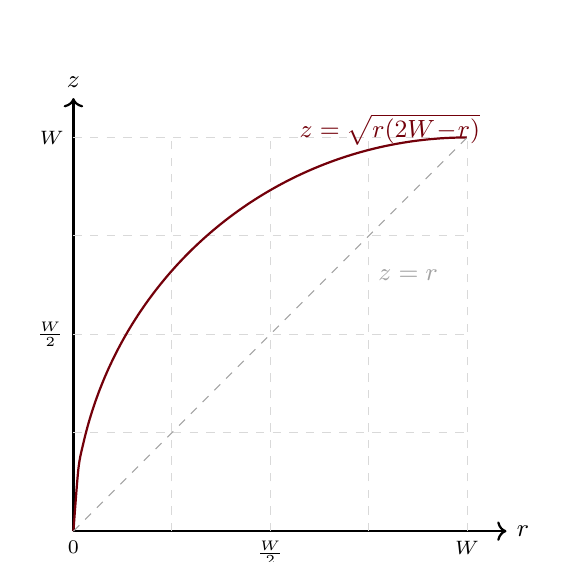
\begin{tikzpicture}[scale=5]
% Axes
\draw[->, thick] (0,0) -- (1.1,0) node[right, font=\small] {$r$};
\draw[->, thick] (0,0) -- (0,1.1) node[above, font=\small] {$z$};
% Grid
\foreach \v in {0.25,0.5,0.75,1.0} {
  \draw[dashed, gray!30] (\v,0) -- (\v,1);
  \draw[dashed, gray!30] (0,\v) -- (1,\v);
}
% Tick labels
\node[below, font=\scriptsize] at (0,0) {$0$};
\node[below, font=\scriptsize] at (0.5,0) {$\frac{W}{2}$};
\node[below, font=\scriptsize] at (1,0) {$W$};
\node[left, font=\scriptsize] at (0,0.5) {$\frac{W}{2}$};
\node[left, font=\scriptsize] at (0,1) {$W$};
% Quarter-circle arc: z = sqrt(r(2-r)), r in [0,1]
\draw[thick, USC_Garnet, domain=0:1, samples=80, smooth] plot (\x, {sqrt(\x*(2-\x))});
% Identity line
\draw[dashed, USC_Black50] (0,0) -- (1,1);
% Labels
\node[USC_Garnet, font=\small\bfseries, anchor=west] at (0.55,1.02) {$z = \sqrt{r(2W\!-\!r)}$};
\node[USC_Black50, font=\small, anchor=west] at (0.75,0.65) {$z = r$};
\end{tikzpicture}
\end{center}
The curve is a quarter-circle arc from $(0,0)$ to $(W,W)$, lying above the identity line, indicating the transformation boosts lower intensities.
\end{stepbox}

\begin{resultsbox}
The transformation that maps the input PDF $p_r(r)$ to the desired output PDF $p_z(z)$ is:
\[
z = f(r) = \sqrt{r\bigl(2(L-1) - r\bigr)}, \qquad 0 \leq r \leq L-1
\]
This is a quarter-circle arc from $(0,0)$ to $(L\!-\!1,\, L\!-\!1)$. $\blacksquare$
\end{resultsbox}


% ============================================================================
% END OF DOCUMENT
% ============================================================================

\end{document}
